% Options for packages loaded elsewhere
\PassOptionsToPackage{unicode}{hyperref}
\PassOptionsToPackage{hyphens}{url}
%
\documentclass[
]{article}
\usepackage{lmodern}
\usepackage{amssymb,amsmath}
\usepackage{ifxetex,ifluatex}
\ifnum 0\ifxetex 1\fi\ifluatex 1\fi=0 % if pdftex
  \usepackage[T1]{fontenc}
  \usepackage[utf8]{inputenc}
  \usepackage{textcomp} % provide euro and other symbols
\else % if luatex or xetex
  \usepackage{unicode-math}
  \defaultfontfeatures{Scale=MatchLowercase}
  \defaultfontfeatures[\rmfamily]{Ligatures=TeX,Scale=1}
\fi
% Use upquote if available, for straight quotes in verbatim environments
\IfFileExists{upquote.sty}{\usepackage{upquote}}{}
\IfFileExists{microtype.sty}{% use microtype if available
  \usepackage[]{microtype}
  \UseMicrotypeSet[protrusion]{basicmath} % disable protrusion for tt fonts
}{}
\makeatletter
\@ifundefined{KOMAClassName}{% if non-KOMA class
  \IfFileExists{parskip.sty}{%
    \usepackage{parskip}
  }{% else
    \setlength{\parindent}{0pt}
    \setlength{\parskip}{6pt plus 2pt minus 1pt}}
}{% if KOMA class
  \KOMAoptions{parskip=half}}
\makeatother
\usepackage{xcolor}
\IfFileExists{xurl.sty}{\usepackage{xurl}}{} % add URL line breaks if available
\IfFileExists{bookmark.sty}{\usepackage{bookmark}}{\usepackage{hyperref}}
\hypersetup{
  pdftitle={IDB Data Exercise},
  pdfauthor={Kevin Conklin},
  hidelinks,
  pdfcreator={LaTeX via pandoc}}
\urlstyle{same} % disable monospaced font for URLs
\usepackage[margin=1in]{geometry}
\usepackage{graphicx,grffile}
\makeatletter
\def\maxwidth{\ifdim\Gin@nat@width>\linewidth\linewidth\else\Gin@nat@width\fi}
\def\maxheight{\ifdim\Gin@nat@height>\textheight\textheight\else\Gin@nat@height\fi}
\makeatother
% Scale images if necessary, so that they will not overflow the page
% margins by default, and it is still possible to overwrite the defaults
% using explicit options in \includegraphics[width, height, ...]{}
\setkeys{Gin}{width=\maxwidth,height=\maxheight,keepaspectratio}
% Set default figure placement to htbp
\makeatletter
\def\fps@figure{htbp}
\makeatother
\setlength{\emergencystretch}{3em} % prevent overfull lines
\providecommand{\tightlist}{%
  \setlength{\itemsep}{0pt}\setlength{\parskip}{0pt}}
\setcounter{secnumdepth}{-\maxdimen} % remove section numbering
\usepackage{booktabs}
\usepackage{longtable}
\usepackage{array}
\usepackage{multirow}
\usepackage{wrapfig}
\usepackage{float}
\usepackage{colortbl}
\usepackage{pdflscape}
\usepackage{tabu}
\usepackage{threeparttable}
\usepackage{threeparttablex}
\usepackage[normalem]{ulem}
\usepackage{makecell}
\usepackage{xcolor}
\usepackage{siunitx}
\newcolumntype{d}{S[input-symbols = ()]}

\title{IDB Data Exercise}
\author{Kevin Conklin}
\date{4/26/2022}

\begin{document}
\maketitle

\hypertarget{i.-load-ratings-data}{%
\subsubsection{I. Load Ratings Data}\label{i.-load-ratings-data}}

We start the project by loading in the ratings data and verifying the
shape of the data. This data will be the basis of our analysis. To
ensure everything looks good, we will verify the number of observations,
variables, and unique respondents in the data.

\begin{verbatim}
## [1] "There are 18189 observations, 4 variables, and 1056 unique respondents in the Ratings dataset."
\end{verbatim}

\hypertarget{ii.-duplicate-cleaning}{%
\subsubsection{II. Duplicate Cleaning}\label{ii.-duplicate-cleaning}}

Before running analysis on the ratings survey file, it was important to
review any duplicates in the data. There appears to have been 257 set of
duplicates. For each set of duplicates, there were no more than two
observations. I have removed the dupliucates by selecting only the first
response for a particular worker and aspect.

\hypertarget{iii.-analysis-of-subjective-riches}{%
\subsubsection{III. Analysis of Subjective
Riches}\label{iii.-analysis-of-subjective-riches}}

Subjective riches is a summary metric used to describe the overall
satisfaction of a respondent with each of the aspects referred to in the
survey. It was calculated by averaging the ratings given to all aspects
for a given individual. The table below gives an overview of the spread
of subjective riches in the data set. The average and median ratings are
about 61, although they range from a little over 5 to 100 across the
1056 individuals that responded. From the histogram, we can see that the
scores have a unimodal and bell-curve distribution, with the exception
of the truncation right at a rating of 100 (the highest rating
possible).

\begin{wraptable}{l}{0pt}

\caption{\label{tab:subjective_riches}<span style='font-size:20px'>Subjective Riches Descriptive Statistics</span>}
\centering
\begin{tabular}[t]{l|l}
\hline
Statistic Name & Value\\
\hline
Number of Respondents & 1056\\
\hline
Minimum & 5.8\\
\hline
25th Percentile & 49.1\\
\hline
50th Percentile & 61.4\\
\hline
75th Percentile & 75.1\\
\hline
Maximum & 100\\
\hline
Mean & 61.6\\
\hline
Standard Deviation & 19\\
\hline
\multicolumn{2}{l}{\rule{0pt}{1em}\textsuperscript{a} Subjective Riches is calculated using the average rating  17 aspects}\\
\multicolumn{2}{l}{\rule{0pt}{1em}\textsuperscript{b} These descriptive statistics are based on a sample of 1056 respondants}\\
\end{tabular}
\end{wraptable}

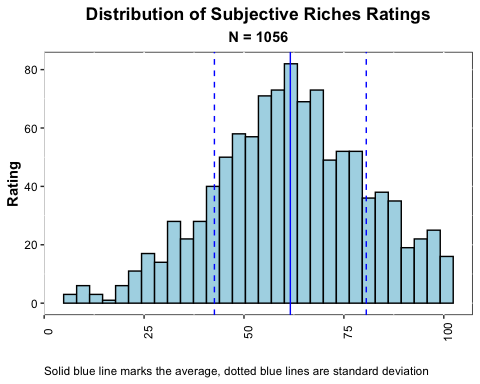
\includegraphics[width=0.5\linewidth]{IDB_Test_Script_files/figure-latex/subjective_riches-1}

\hypertarget{iv.-load-demographic-data}{%
\subsubsection{IV. Load Demographic
Data}\label{iv.-load-demographic-data}}

Before proceeding to the regression analysis, we will need to combine
the demographic data and the subjective riches data. We can see that the
dataset has 1056 unique respondents, just as we saw in the ratings data
set. There are 1056 observations, which implies that each unique
respondent has only one observation. We also have six variables in the
data set. From here we can feel comfortable merging our two data sets.

\begin{verbatim}
## [1] "There are 1056 observations, 6 variables, and 1056 unique respondents in the Demographics dataset."
\end{verbatim}

\hypertarget{v.-regression-analysis}{%
\subsubsection{V. Regression Analysis}\label{v.-regression-analysis}}

To better understand the relationship between demographics and
subjective riches, we will run two regressions. The first will be a
simple bivariate regression of subjective riches over income. The second
will be a multivariate regression that will analyze the relationship
between income and subjective riches holding for age, gender, education,
and race. Note that in both regressions I have converted income into the
natural log of income. This helps to deal with issues of
nonlinearity,and also improves interpretation.

From the simple bivariate regression, we can see that income does have a
significant positive relationship with subjective riches. A one percent
increase in income is associated with a 0.0499 unit unit increase in the
subjective riches rating. This relationship is significant at the 0.1\%
level. The size of the relationship is not necessarily very large. It
implies that a 100\% increase in income would only increase subjective
riches by about 5, compared to a standard deviation of 19. The intercept
of the regression implies that an individual with no income would have,
on average, a subjective riches rating of 8.19, although this is not
very meaningful given the smallest income in the data set is \$10K.

The multivariate regression gives surprisingly similar results, despite
the addition of so many controls. I have only displayed the coefficients
that were statistically significant at at least the 5\% level. This left
only gender and income. Age, race, and education were not significantly
related to the subjective riches rating holding for other model factors,
even after running join significance tests.

Despite the controls, the coefficient for log of income stayed very
similar. In this regression, holding race, gender, age, education
constant, a one percent increase in income is associated with a 0.0477
increase in the subjective riches rating. Once again, this coefficient
is significant at the 0.1\% level. We also see that gender has a
significant relationship with the subjective riches rating. On average,
men have a subjective riches rating that is 2.77 points higher than
females of the same race, educational attainment, age, and income. This
relationship is significant at the 5\% level. The fact that the
coefficient stayed so consistent is a bit surprising, but may be due to
the very low correlations between variables, as shown in the correlation
matrix.

The slight decrease in the coefficient for log of income may have been
due to the positive correlation between income and being male. Since
males have higher incomes and higher subjective riches ratings on
average, omitting it from the regression likely caused a slight upward
bias on the coefficient. From this analysis we can conclude that income
is very likely related to subjective riches ratings. However, the
R-squared values of the first and second models are only .04 and .06
respectively. In other words, income only explains about 4\% of the
variation in subjective riches. More analysis would be needed to better
understand it.

If I were to be given household size, I might create a new variable that
would be the income divided by the size of the household. This would be
done under the assumption that the respondent is the main money earner
in the household, and might give a better idea of the financial
resources available per person. I would add the household size as a
control variable as well.

\begin{center}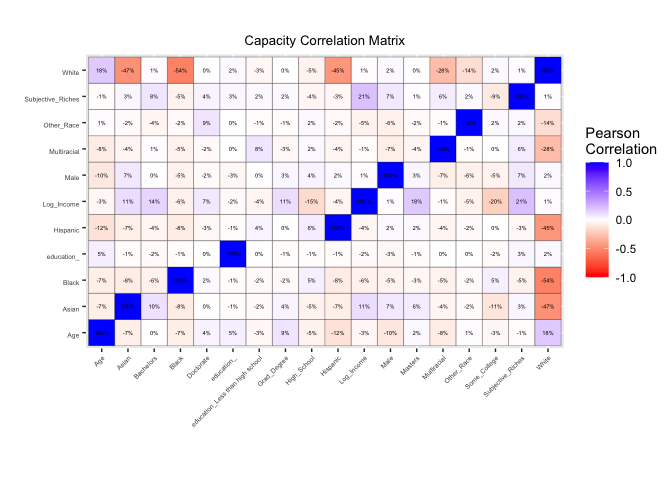
\includegraphics{IDB_Test_Script_files/figure-latex/ols-1} \end{center}

\begin{table}

\caption{\label{tab:ols}Subjective Riches Regression}
\centering
\begin{tabular}[t]{lccc}
\toprule
  & (Intercept) & Log\_Income & Male\\
\midrule
Model 1 & \num{8.192} & \num{4.994}*** & \\
 & (\num{7.857}) & (\num{0.732}) & \\
Model 2 & \num{25.436}* & \num{4.779}*** & \num{2.772}*\\
 & (\num{12.468}) & (\num{0.777}) & (\num{1.179})\\
\bottomrule
\multicolumn{4}{l}{\rule{0pt}{1em}Only signficant coefficients displayed}\\
\multicolumn{4}{l}{\rule{0pt}{1em}+ p $<$ 0.1, * p $<$ 0.05, ** p $<$ 0.01, *** p $<$ 0.001}\\
\end{tabular}
\end{table}

\hypertarget{v.-scatter-plot}{%
\subsubsection{V. Scatter Plot}\label{v.-scatter-plot}}

If I were to create a scatter plot showing the relationship between
subjective ratings of health, income, and age, I would do the following
three steps:

\begin{enumerate}
\def\labelenumi{\arabic{enumi}.}
\tightlist
\item
  I would create a health specific index by averaging together the
  ratings on health related aspects, such as:
\end{enumerate}

\begin{itemize}
\tightlist
\item
  the quality of your sleep
\item
  you not feeling anxious
\item
  your emotional stability
\item
  your health
\item
  your mental health
\item
  your physical fitness
\end{itemize}

\begin{enumerate}
\def\labelenumi{\arabic{enumi}.}
\setcounter{enumi}{1}
\item
  I would then break age into quantiles - which will make the categories
  easier to visualize
\item
  I would also divide income by 1000 to report income in thousands,
  which might make the numbers easier to read
\item
  Finally, I would make my scatter plot by plotting income on the
  x-axis, subjective health on the y-axis, and would shade points a
  specific color based on their age category, which might help to show
  age groupings.
\end{enumerate}

\begin{center}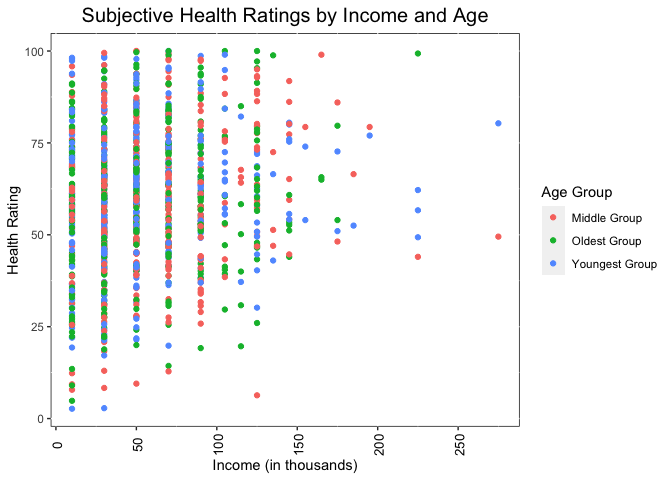
\includegraphics{IDB_Test_Script_files/figure-latex/scatter_build-1} \end{center}

\hypertarget{vi.-conclusions}{%
\subsubsection{VI. Conclusions}\label{vi.-conclusions}}

From both the regression analysis and the scatter plot, we can see that
income plays a role in subjective well-being, but maybe not as large a
role as would have been expected. According to the regression model,
gender also plays a role in determining subjective well-being. One of
the main conclusions I've drawn from this exercise is how much we cannot
explain about variations in subjective well-being. Even with the
multivariate regression, only about 6\% of the variation in subjective
well-being.

There might be a few reasons that we are not seeing results. One reason
might be specification. For instance, income may have differing impacts
for different groups. Including interactions with gender, age, race, or
education variables might allow for a more robust understanding of the
relationship between income and subjective well-being.

Another issue might be how we are defining subjective well-being. In the
subjective wellness metric, we are combining ratings for a pretty wide
array of aspects. It could certain demographic attributes apply to some
aspects and not others, or to different aspects in different ways. To
some extent this was addressed in the scatter plot by focusing on health
specific questions, but even this grouping was done somewhat
subjectively. One solution might be to run exploratory factor analysis
on the aspect ratings. That might help us to find underlying groupings
based on the covariance in the data. Then we could focus on regressions
of demographics on these specific groupings, which might yield better
results.

The last issue is just how the survey itself was collected. Not very
much context was given around how to rate aspects. Due to its subjective
nature, people may not always answer in the same way. A 70 to one person
may be equivalent to another person's 50. It might be helpful to use
more objective questions, especially around health and anxiety. ``How
many days in the past week did you have difficulty sleeping?'' for
instance might be a clearer way to get at the ``quality of your sleep''
aspect.

\end{document}
